\documentclass[border=8pt,12pt]{standalone}
\usepackage[scaled]{helvet}
\usepackage[T1]{fontenc}
\renewcommand\familydefault{\sfdefault}

\usepackage{tikz}
\usetikzlibrary{arrows.meta, positioning}

\definecolor{knowFill}{HTML}{EAF1F7}
\definecolor{knowLine}{HTML}{315C86}
\definecolor{divFill}{HTML}{E6EBD2}
\definecolor{divLine}{HTML}{6F7F3D}
\definecolor{belongLine}{HTML}{333333}
\definecolor{belongFill}{HTML}{F7F4EC}
\definecolor{warn}{HTML}{B3261E}

\begin{document}

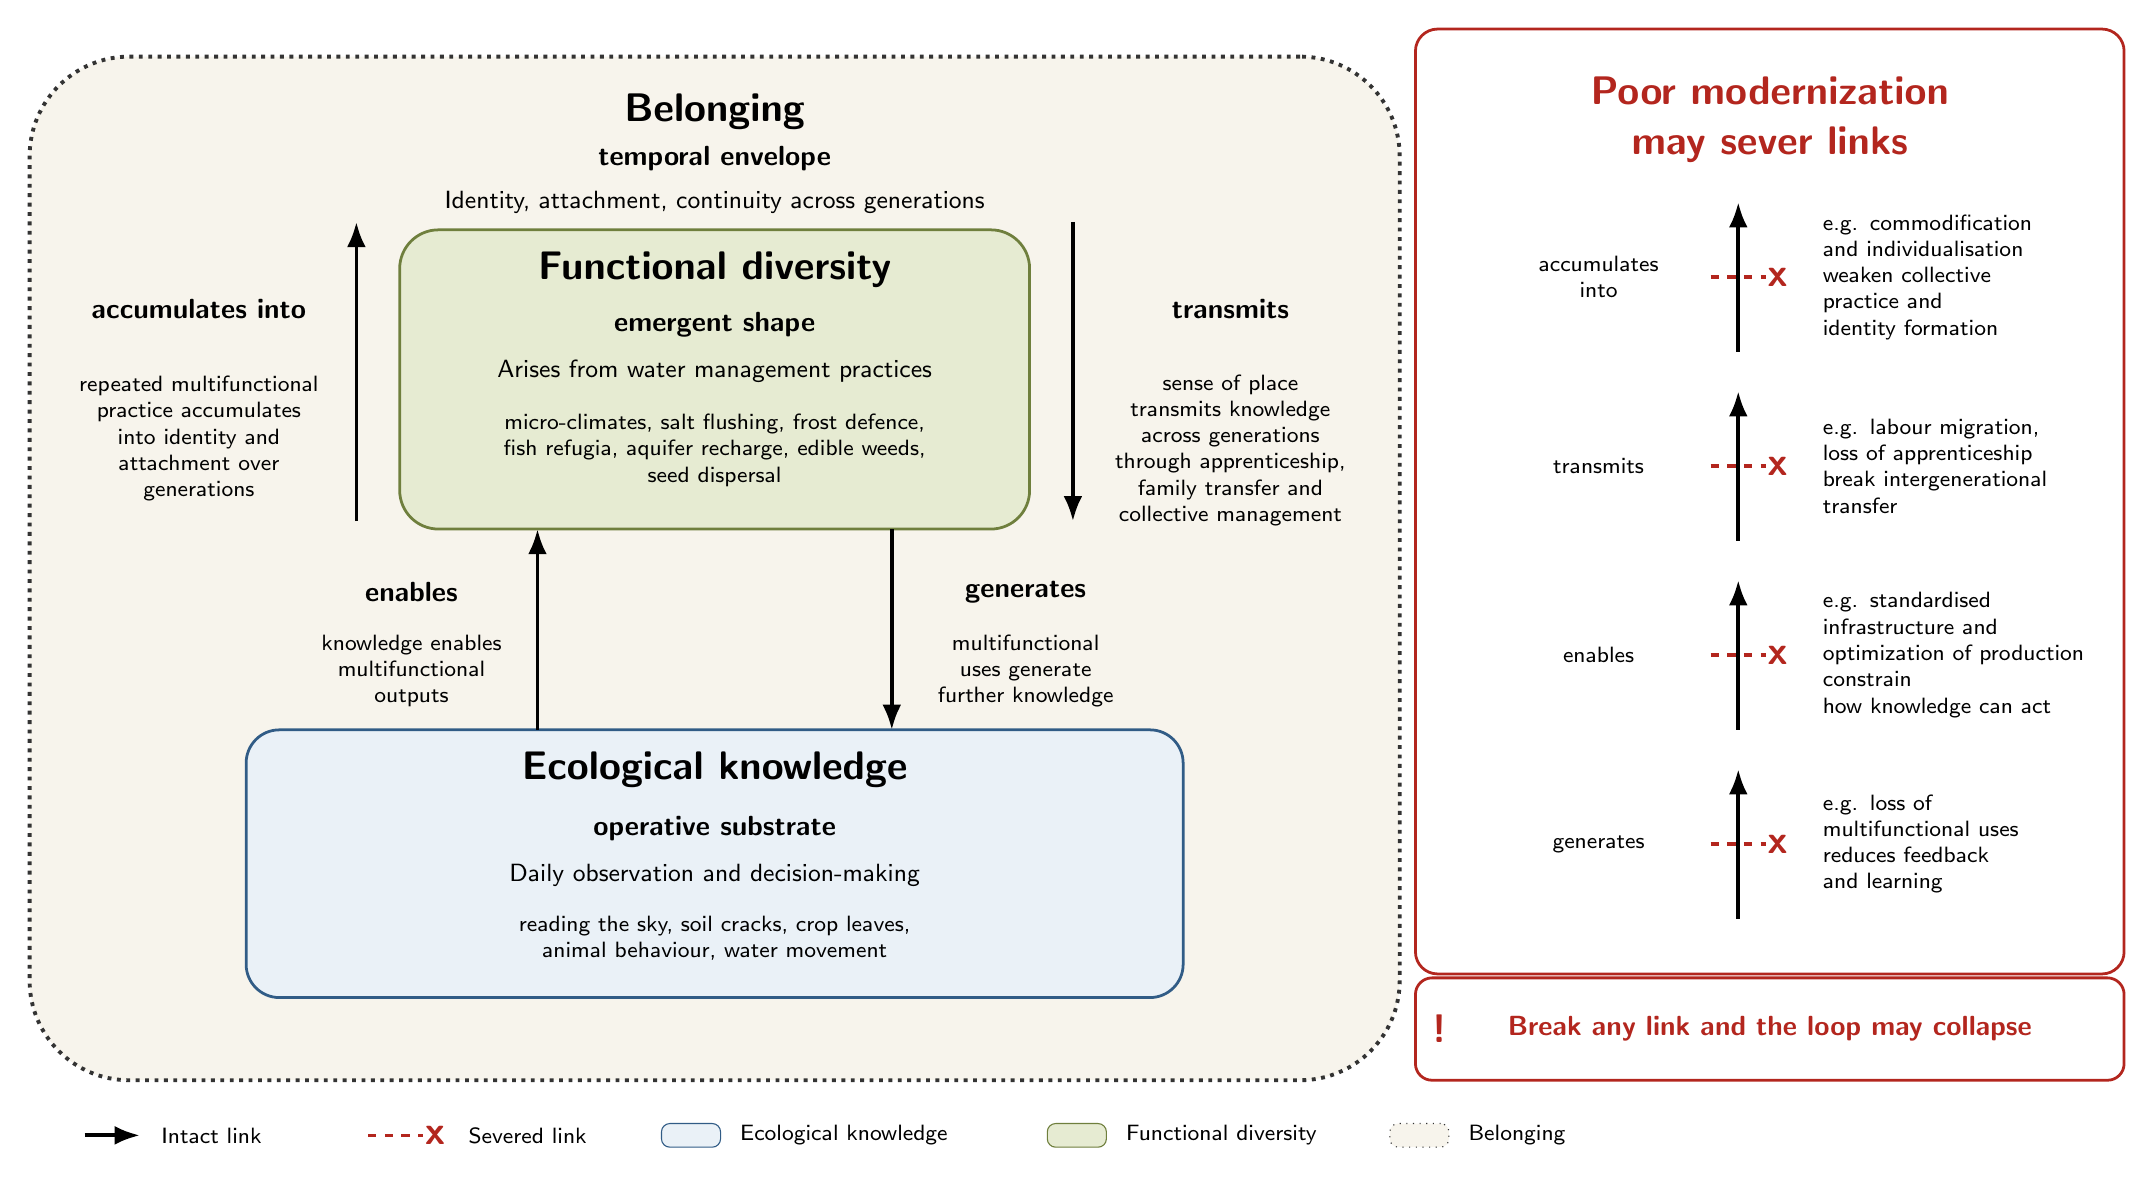
\begin{tikzpicture}[
  font=\sffamily,
  >=Latex,
  title/.style={font=\bfseries\Large, align=center},
  subtitle/.style={font=\bfseries\normalsize, align=center},
  body/.style={font=\small, align=center},
  note/.style={font=\footnotesize, align=center},
  flow/.style={->, line width=1.35pt},
  sever/.style={warn, dashed, line width=1.2pt},
  xmark/.style={warn, font=\bfseries\Large}
]

% =========================================================
% MAIN ARTICULATION
% =========================================================

\node[
  draw=belongLine,
  fill=belongFill,
  dotted,
  line width=1.4pt,
  rounded corners=36pt,
  minimum width=17.4cm,
  minimum height=13.0cm
] (belongBox) at (0,0) {};

\node[title] at (0,5.80) {Belonging};
\node[subtitle] at (0,5.20) {temporal envelope};
\node[body] at (0,4.65) {Identity, attachment, continuity across generations};

% Functional diversity
\node[
  draw=divLine,
  fill=divFill,
  rounded corners=14pt,
  line width=1pt,
  minimum width=8.0cm,
  minimum height=3.80cm
] (diversity) at (0,2.40) {};

\node[title] at (0,3.80) {Functional diversity};
\node[subtitle] at (0,3.10) {emergent shape};
\node[body] at (0,2.50)
{Arises from water management practices};

\node[note, text width=7.50cm] at (0,1.50)
{micro-climates, salt flushing, frost defence,\\fish refugia, aquifer recharge, edible weeds,\\seed dispersal};

% Ecological knowledge
\node[
  draw=knowLine,
  fill=knowFill,
  rounded corners=12pt,
  line width=1pt,
  minimum width=11.9cm,
  minimum height=3.40cm
] (knowledge) at (0,-3.75) {};

\node[title] at (0,-2.55) {Ecological knowledge};
\node[subtitle] at (0,-3.30) {operative substrate};
\node[body, text width=10.6cm] at (0,-3.90)
{Daily observation and decision-making};

\node[note, text width=10.6cm] at (0,-4.70)
{reading the sky, soil cracks, crop leaves,\\animal behaviour, water movement};

% =========================================================
% FLOWS: CENTER PAIR
% =========================================================

% Knowledge -> diversity
\draw[flow] (-2.25,-2.05) -- (-2.25,0.50);
\node[subtitle] (s_enables) at (-3.85,-0.30) {enables};
\node[note, text width=3.50cm] at (-3.85,-1.30)
{knowledge enables\\multifunctional\\outputs};

% Diversity -> knowledge
\draw[flow] (2.25,0.50) -- (2.25,-2.05);
\node[subtitle] (s_generates) at (3.95,-0.30) {generates};
\node[note, text width=3.60cm] at (3.95,-1.30)
{multifunctional\\uses generate\\further knowledge};

% =========================================================
% FLOWS: OUTER PAIR
% =========================================================

% Diversity -> belonging
\draw[flow] (-4.55,0.60) -- (-4.55,4.40);
\node[subtitle] (s_acc) at (-6.55,3.30) {accumulates into};
\node[note, text width=3.70cm] at (-6.55,1.65)
{repeated multifunctional\\practice accumulates\\into identity and\\attachment over\\generations};

% Belonging -> knowledge
\draw[flow] (4.55,4.40) -- (4.55,0.60);
\node[subtitle] (s_trans) at (6.55,3.30) {transmits};
\node[note, text width=3.70cm] at (6.55,1.50)
{sense of place\\transmits knowledge\\across generations\\through apprenticeship,\\family transfer and\\collective management};


% =========================================================
% MODERNISATION PANEL
% =========================================================

\node[
  draw=warn,
  rounded corners=8pt,
  line width=1pt,
  minimum width=9.0cm,
  minimum height=12.0cm
] (modern) at (13.40,0.85) {};

\node[warn, font=\bfseries\Large, align=center] at (13.40,5.70)
{Poor modernization\\may sever links};

% Broken links inside panel
\foreach \y/\lab/\txt in {
  3.70/{accumulates\\into}/{commodification\\and individualisation\\weaken collective\\practice and\\identity formation},
  1.30/{transmits}/{labour migration,\\loss of apprenticeship\\break intergenerational\\transfer},
  -1.10/{enables}/{standardised\\infrastructure and\\optimization of production constrain\\ how knowledge can act},
  -3.50/{generates}/{loss of\\multifunctional uses\\reduces feedback\\and learning}
}{
  \draw[flow] (13.00,\y-0.95) -- (13.00,\y+0.95);
  \draw[sever] (12.65,\y) -- (13.35,\y);
  \node[xmark] at (13.50,\y) {x};

  \node[note, text width=2.2cm, anchor=east] at (12.45,\y) {\lab};

  \node[note, text width=3.50cm, anchor=west, align=left] at (13.95,\y)
  {e.g. \txt};
}

% Warning box
\node[
  draw=warn,
  rounded corners=6pt,
  line width=1pt,
  minimum width=9.0cm,
  minimum height=1.30cm
] at (13.40,-5.85) {};

\node[warn, font=\bfseries\normalsize, align=center] at (13.40,-5.85)
{Break any link and the loop may collapse};

\node[warn, font=\bfseries\Large] at (9.20,-5.85) {!};

% =========================================================
% LEGEND
% =========================================================

\draw[flow] (-8.0,-7.20) -- (-7.3,-7.20);
\node[note, anchor=west] at (-7.15,-7.20) {Intact link};

\draw[sever] (-4.4,-7.20) -- (-3.7,-7.20);
\node[xmark] at (-3.55,-7.20) {x};
\node[note, anchor=west] at (-3.25,-7.20) {Severed link};

\node[
  draw=knowLine,
  fill=knowFill,
  rounded corners=3pt,
  minimum width=0.75cm,
  minimum height=0.30cm
] at (-0.30,-7.20) {};
\node[note, anchor=west] at (0.20,-7.20) {Ecological knowledge};

\node[
  draw=divLine,
  fill=divFill,
  rounded corners=3pt,
  minimum width=0.75cm,
  minimum height=0.30cm
] at (4.60,-7.20) {};
\node[note, anchor=west] at (5.10,-7.20) {Functional diversity};

\node[
  draw=belongLine,
  fill=belongFill,
  dotted,
  rounded corners=3pt,
  minimum width=0.75cm,
  minimum height=0.30cm
] at (8.95,-7.20) {};
\node[note, anchor=west] at (9.45,-7.20) {Belonging};

\end{tikzpicture}

\end{document}

